%Matteo Kumar - Leonhard Schatt
% Fortgeschrittenes Physikalisches Praktikum

% Teilauswertung CD

\section{Untersuchung eines CD-Presswerkzeugs}
\subsection{Bumphöhe}

Zunächst wird der 50$\mu m$-Ausschnitt zur Bestimmung der Bumphöhe untersucht.
Auf Abb. \ref{bild:CD50Linie} ist ein großer heller Fleck am unteren Bildrand zu erkennen. Dies könnte eine Verunreinigung wie z.B. Staub sein. 
Zur Bestimmung der Höhe der Bumps wird das Profil über mehrere Tracks betrachtet. 

\begin{figure}[h]
    \centering
    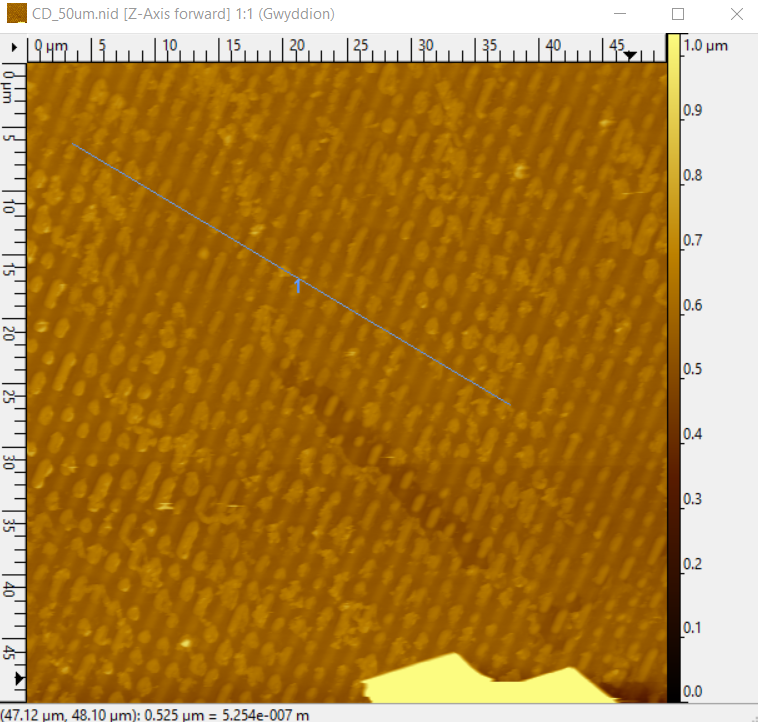
\includegraphics[scale = 0.47]{Bilder/CD50Linie.png}
    \caption{Aufnahme eines CD-Pressswerkzeugs auf 50x50 $\mu$m. Unten ist eine Verunreinigung als heller Fleck zu sehen. Die Strecke 
    für das benutzte Höhenprofil ist ebenfalls eingezeichnet}
    \label{bild:CD50Linie}
\end{figure}

\begin{figure}[h]
    \centering
    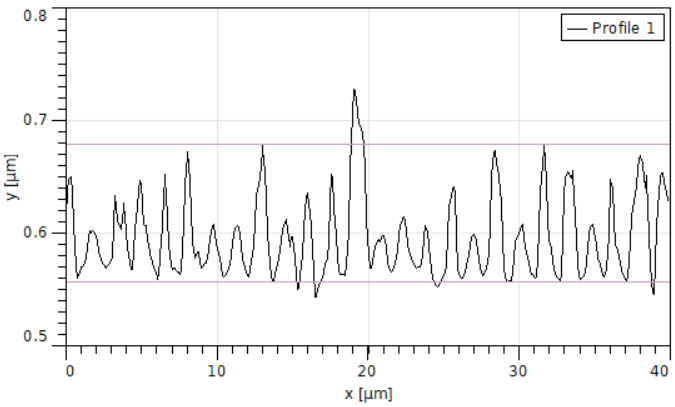
\includegraphics[scale = 0.6]{Bilder/CD50Profil.png}
    \caption{Höhenprofil durch die Bumps des CD-Presswerkzeuges. Als Anhaltspunkt für die Höhe der Bumps dienen die rosafarbenen Linien, die 
    122.2 nm auseinander sind.}
    \label{bild:CD50Profil}
\end{figure}

Die Höhe der Bumps soll mit Hilfe von Abb. \ref{bild:CD50Profil} eingeordnet werden. 
Die rosanen Linien stellen einen Abstand von 122.2 nm dar. Der große Bump hat eine Höhe von 164.4 nm. Der Hersteller 
gibt allerdings Höhen von ca. 200nm an (\cite{SampleKit2007}). Da die Ungenauigkeit des Herstellerwertes nicht bekannt ist, ist eine Einordnung an dieser Stelle 
schwierig. Allerdings ist durchaus zu erkennen, dass die gemessenen Bumps deutlich kleiner sind. Womöglich liegt auch hier bereits eine 
Abnutzung von einigen nm vor.
\newpage

\subsection{Trackabstand}

Nun wird der 20$\mu m$-Ausschnitt betrachtet. Es wird ein Höhenprofil entlang der in Abb. \ref{bild:CD20Linie} eingezeichneten Strecke 
erstellt. Zur Bestimmung des Trackabstandes wird das gesamte Profil über 12 Bumps hinweg gemessen, wie in Abb. \ref{bild:CD20Profil} zu 
sehen. 

\begin{figure}[h]
    \centering
    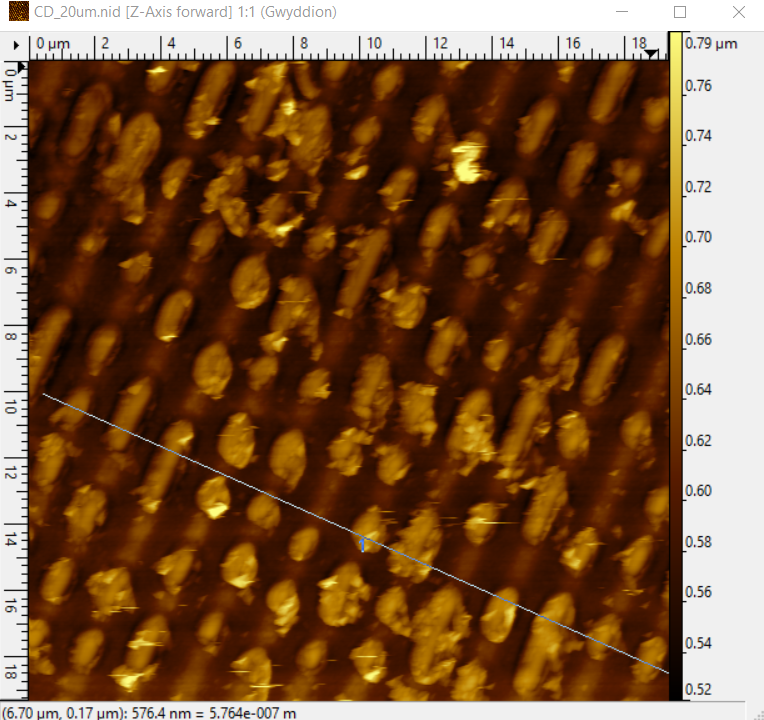
\includegraphics[scale = 0.5]{Bilder/CD20Linie.png}
    \caption{Aufnahme eines CD-Pressswerkzeugs auf 20x20 $\mu$m. Die Strecke 
    für das benutzte Höhenprofil ist ebenfalls eingezeichnet}
    \label{bild:CD20Linie}
\end{figure}

\begin{figure}[h]
    \centering
    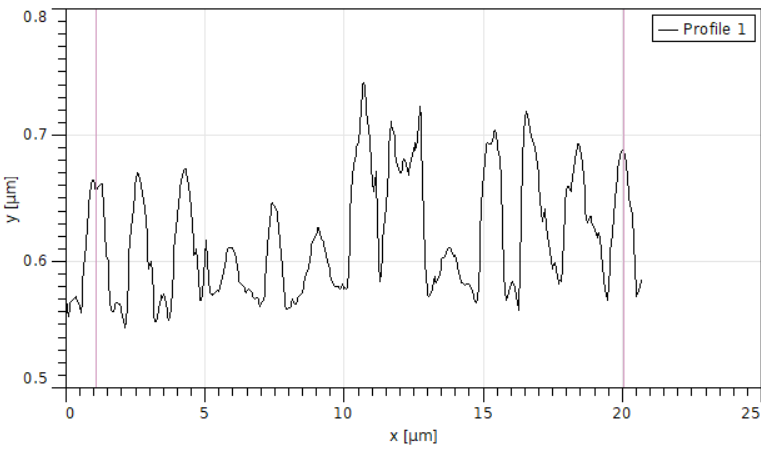
\includegraphics[scale = 0.6]{Bilder/CD20Profil.png}
    \caption{Profil durch die Bumps des Presswerkzeugs. Zur Ermittlung der Trackbreite wurde über 12 Bumps zwischen den rosafarbenen 
    Linien gemessen.}
    \label{bild:CD20Profil}
\end{figure}


Die rosanen Linien stellen einen Abstand von 18.981 $\mu$m dar. Das entspricht einem Trackabstand von $d_{Tr} = 1.582 \mu m$.
Der Fehler ergibt sich aus der Wahl der Veressungslinien, da die Mitte der Bumps nicht exakt bestimmt werden konnte, da die Spitzen und 
der Mittelpunkt zwischen Anstieg und Abfall der Bumps nicht immer übereinstimmen. Deshalb wird der Fehler für beide Linien anhand des 
Profils auf jeweils 0.3 $\mu$m geschätzt. Dies entspricht einem Fehler von 0.05 $\mu$m für den Mittelwert, wodurch sich für den Gesamtfehler ergibt: 
\begin{equation*}
    s = \sqrt{0.05^2 + (1.58 \cdot 0.012)^2}\, \mu m = 0.053\, \mu m
\end{equation*}

Damit ergibt sich der Trackabstand zu

\begin{equation*}
    \textcolor{red}{d_{Tr} = (1.58 \pm 0.06) \mu m}.
\end{equation*}

Der Hersteller gibt einen nominellen Wert von 1.6$\mu$m an (\cite{SampleKit2007}). 
Dieser liegt innerhalb des Fehlers; er wird also durch die Messung bestätigt.

\subsection{Bumplänge}

Als nächstes werden die Längen der Bumps ausgemessen. Dazu wird ein Höhenprofil entlang eines Tracks, wie in Abb. \ref{bild:CD20Laenge} 
gezeigt, angelegt.  

\begin{figure}[h]
    \centering
    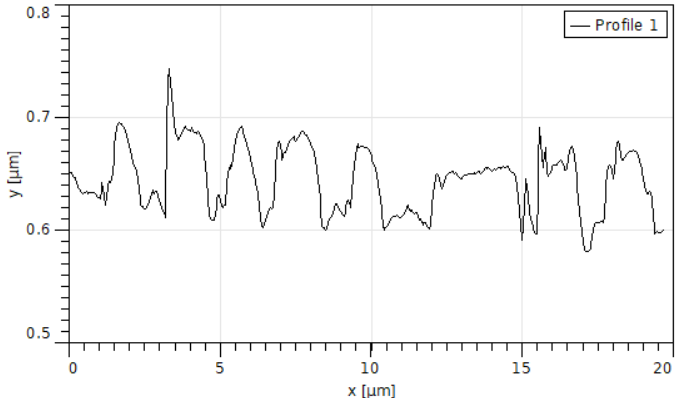
\includegraphics[scale = 0.8]{Bilder/CD20LaengeProfil.png}
    \caption{Profil durch die Bumps des Presswerkzeugs in Längsrichtung.}
    \label{bild:CD20LaengeProfil}
\end{figure}


\begin{figure}[h]
    \centering
    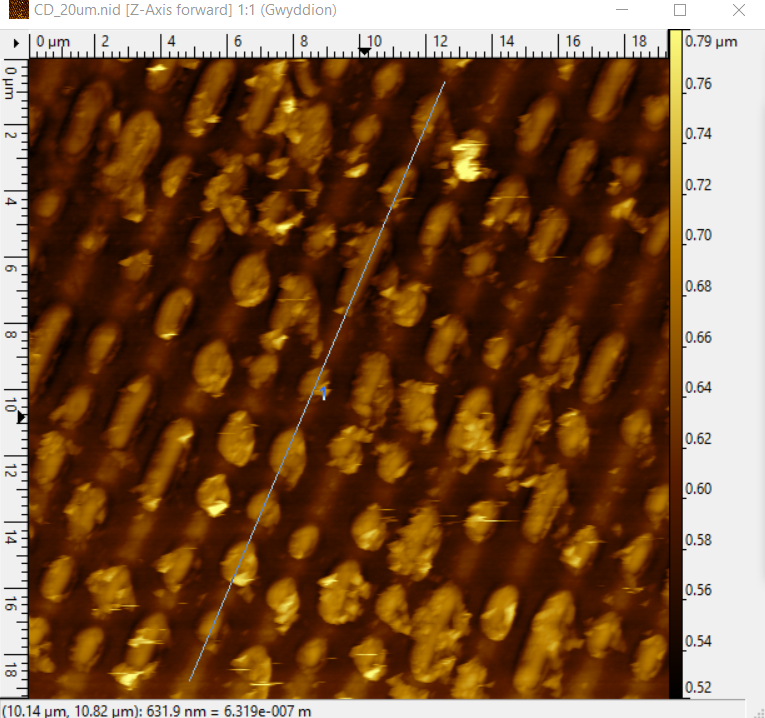
\includegraphics[scale = 0.5]{Bilder/CD20Laenge.png}
    \caption{Strecke entlang eines Tracks, entlang der das Profil zur Bestimmung der Länge der Bumps ermittelt wird.}
    \label{bild:CD20Laenge}
\end{figure}


\newpage

Auf diesem Profil (Abb. \ref{bild:CD20LaengeProfil}) sind acht größere Bumps erkennbar. Von links nach rechts 
sind deren Längen: 

\begin{center}
    \centering
    \begin{tabular}{l|r}
        Nummer Bump (v.l.n.r.) & Länge / $\mu$m \\
        \hline
        1 & 1.28 $\pm$ 1\\
        2 & 1.66 $\pm$ 1\\
        3 & 1.45 $\pm$ 1\\
        4 & 1.95 $\pm$ 1\\
        5 & 1.33 $\pm$ 1\\
        6 & 3.11 $\pm$ 1\\
        7 & 1.74 $\pm$ 1\\
        8 & 1.82 $\pm$ 1\\
        
    \end{tabular}
\end{center}

Die Längen der Bumps in dieser Auswahl liegen also alle im Bereich von 1.2-3.2$\mu$m. Laut Hersteller sollten die Längen in einer Spanne von 
0.8-3$\mu$m liegen (\cite{SampleKit2007}). 
Berücksichtigt man noch die Fehler beim Setzen der Markierungen beim Ausmessen der Bumps (abgeschätzt auf 1$\mu$m 
pro Markierung), so umfasst der angegebene Bereich noch die gemessenen Werte. 
\clearpage